\documentclass{sig-alternate}

\usepackage[utf8]{inputenc}
\usepackage[T1]{fontenc}
\usepackage[english]{babel}
\usepackage{amsmath}
\usepackage{ae}
\usepackage{icomma}
\usepackage{units}
\usepackage{color}
\usepackage{graphicx}
\usepackage{epstopdf}
\usepackage{subfigure}
\usepackage{natbib}
\usepackage{pgfplots}
\usepackage{multirow}
% Sub- and superscript
\newcommand{\superscript}[1]{\ensuremath{^{\textrm{#1}}}}
\newcommand{\subscript}[1]{\ensuremath{_{\textrm{#1}}}}

%%%%%%%%%%%%%%%%%%%%%%%%%%%%%%%%%%%%%%%%%%%%%%%%%%%%%%%%%%%%
% some commands for commenting
\usepackage{ifthen}
\usepackage{amssymb}
\usepackage[normalem]{ulem} % for \sout
\newboolean{showcomments}
\setboolean{showcomments}{true} % toggle to show or hide comments
\ifthenelse{\boolean{showcomments}}
  {
%\usepackage{showkeys} %Show lables and refs
\newcommand{\nbb}[2]{
% \fbox{\bfseries\sffamily\scriptsize#1}
\fcolorbox{black}{yellow}{\bfseries\sffamily\scriptsize#1}
{\sf$\blacktriangleright$\textcolor{blue}{\textit{#2}}$\blacktriangleleft$}
% \marginpar{\fbox{\bfseries\sffamily#1}}
}
\newcommand{\version}{\emph{\scriptsize$-$9.2.2011$-$}}
\newcommand{\remarks}[1]{\color{red}[#1]\color{black}}
\newcommand{\copied}[1]{\color{green}[#1]\color{black}}
\newcommand{\modified}[1]{\color{blue}[#1]\color{black}}
\newcommand{\raw}{$\rightarrow$}
\newcommand{\ins}[1]{\textcolor{blue}{\uline{#1}}} % please insert
\newcommand{\del}[1]{\textcolor{red}{\sout{#1}}} % please delete
\newcommand{\chg}[2]{\textcolor{red}{\sout{#1}}{\raw}\textcolor{blue}{\uline{#2}}} % please change
\newcommand{\ugh}[1]{\textcolor{red}{\uwave{#1}}} % please rephrase
  }
  {
\newcommand{\nbb}[2]{}
\newcommand{\remarks}[1]{}
\newcommand{\modified}[1]{#1}
\newcommand{\copied}[1]{#1}
\newcommand{\version}{}
\newcommand{\ugh}[1]{#1} % please rephrase
\newcommand{\ins}[1]{#1} % please insert
\newcommand{\del}[1]{} % please delete
\newcommand{\chg}[2]{#2} % please change
  }

\newcommand{\eb}[1]{\nbb{eb}{#1}}
%%%%%%%%%%%%%%%%%%%%%%%%%%%%%%%%%%%%%%%%%%%%%%%%%%%%%%%%%%%%

\graphicspath{{./include/images/}}

\pgfplotsset{
    box plot/.style={
        /pgfplots/.cd,
        black,
        only marks,
        mark=-,
        mark size=1em,
        /pgfplots/error bars/.cd,
        y dir=plus,
        y explicit,
    },
    box plot box/.style={
        /pgfplots/error bars/draw error bar/.code 2 args={%
            \draw  ##1 -- ++(1em,0pt) |- ##2 -- ++(-1em,0pt) |- ##1 -- cycle;
        },
        /pgfplots/table/.cd,
        y index=2,
        y error expr={\thisrowno{3}-\thisrowno{2}},
        /pgfplots/box plot
    },
    box plot top whisker/.style={
        /pgfplots/error bars/draw error bar/.code 2 args={%
            \pgfkeysgetvalue{/pgfplots/error bars/error mark}%
            {\pgfplotserrorbarsmark}%
            \pgfkeysgetvalue{/pgfplots/error bars/error mark options}%
            {\pgfplotserrorbarsmarkopts}%
            \path ##1 -- ##2;
        },
        /pgfplots/table/.cd,
        y index=4,
        y error expr={\thisrowno{2}-\thisrowno{4}},
        /pgfplots/box plot
    },
    box plot bottom whisker/.style={
        /pgfplots/error bars/draw error bar/.code 2 args={%
            \pgfkeysgetvalue{/pgfplots/error bars/error mark}%
            {\pgfplotserrorbarsmark}%
            \pgfkeysgetvalue{/pgfplots/error bars/error mark options}%
            {\pgfplotserrorbarsmarkopts}%
            \path ##1 -- ##2;
        },
        /pgfplots/table/.cd,
        y index=5,
        y error expr={\thisrowno{3}-\thisrowno{5}},
        /pgfplots/box plot
    },
    box plot median/.style={
        /pgfplots/box plot
    }
}

\begin{document}

\title{Automated analysis and planning of social network marketing}
\subtitle{Master's Thesis in Software Engineering}

\numberofauthors{1}
\author{
\alignauthor
Erik Brännström\\
       \affaddr{Chalmers University of Technology}\\
       \email{erikbr@student.chalmers.se}
}

\maketitle

\begin{abstract}
Managing online marketing campaigns is a repetitive and analytical process which is typically done manually by domain experts. This paper deals with the problem of how to use software to manage historical marketing data and use that as a foundation for decision-making with the purpose of optimizing future ad performance.

The solution presented in this thesis involves applying both data mining and automation practices to provide decision makers with knowledge that can be enacted upon. Operators of the system input the historical data, upon which the system creates an estimation model based on said data which is used to estimate the performance of, for the system, previously unseen ads. These suggested ads can either be input by the operator or automatically created by combining existing ad properties.

The solution has been validated on real-world data from an industrial partner in the social networking industry.

\end{abstract}

\keywords{Online marketing, business intelligence, performance estimation, social networks}

% \category{D.1.5}{Programming Techniques}{Object-oriented Programming}
\category{D.2}{Software}{Software Engineering}
\category{I.2.6}{Artificial Intelligence}{Learning}
\category{J.1}{Administrative Data Processing}{Marketing}

% ACM's 2012 Classification Scheme. Unsure of how to style, and no one else seems to use it yet.
%\category{Machine learning}{Learning paradigms}{Supervised learning}
%\category{Computing methodologies}{Software and its engineering}{Software creation and management}{Designing software}{Software implementation planning}{Software design techniques}
%\category{Applied Computing}{Operations research}{Marketing}

\section{Introduction}
As more and more people are using the Internet on a daily basis, the area of online marketing is expanding as a way for organizations to reach large audiences at a relatively low cost. The process of managing the marketing material however requires a lot of manual labor, since results must be properly analyzed and applied to future decisions.

The research in this paper was carried out in association with an industrial partner that relies heavily on online marketing to promote their product to new users. The partner is a social networking company based in Sweden which will be referred to by the name of Company A. The purpose of partnering was to evaluate the prospect of automating parts of the marketing process in a real-world environment and show the validity of the presented solution.

To be able to properly assimilate the contents, the first subsection presents the problem domain and defines useful terminology which is used throughout this paper. These descriptions are relied on in the subsequent two sections, which first details the addressed problem followed by an overview of the solution.

The final section deals with the scope by stating restrictions on what will be covered by this paper.

\subsection{Domain}
This paper exist at the intersection of a number of different areas. As marketing is probably the field furthest from typical software engineering tasks, it will be described in some detail in the first subsection. That will then lead into the concept of business intelligence, followed by a subsection on automation

\subsubsection{Online marketing}
A site that displays advertisement, the publisher, is often paid by the advertiser based on the number of times visitors see or click on the ads, but it may also be coupled with other requirements, such as that the visitor goes on to buy a product from the advertiser in a given time span. The advertisement is generally tailored to the expected interests of the visiting users. This is because advertisers want to keep the costs down while still getting good results and distributors usually prefer to show only relevant information to their visitors to keep them coming back.

A domain description is shown in Figure \ref{fig:MarketingTerminology}. A \emph{marketing campaign}, or simply a \emph{campaign}, is comprised of one or more advertising messages, \emph{ads}, that are directed to one defined audience, the \emph{target} or \emph{target group} (e.g. gender or people searching for certain keywords). Any ad, and by extension campaign, have numeric measures of success called \emph{metrics}. The most commonly used are \emph{impressions}, which is the number of times an ad has been shown, and clicks.

\begin{figure*}[htb] \centering 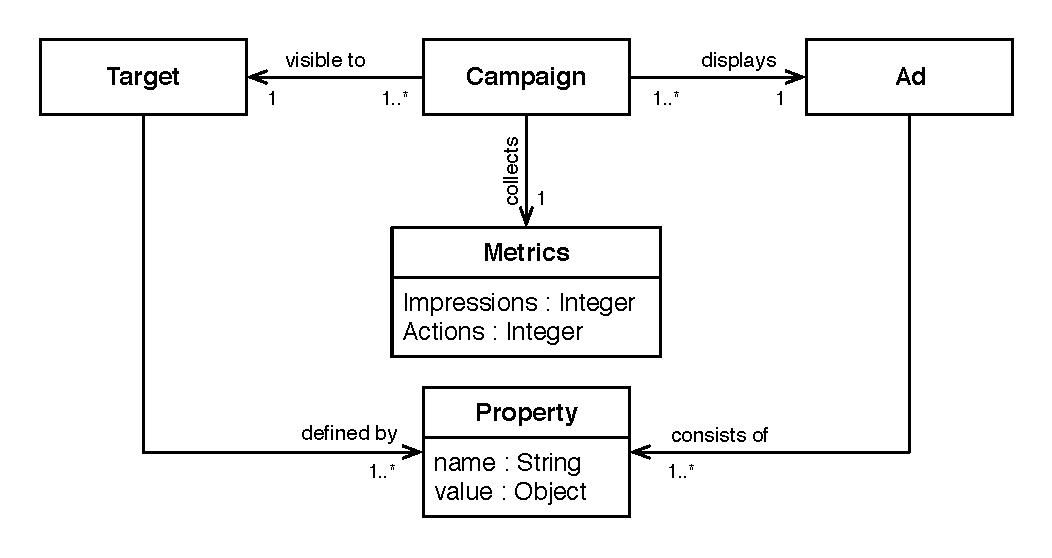
\includegraphics[width=0.58\textwidth]{marketing-uml.eps}
	\caption{UML description of marketing terminology.}
	\label{fig:MarketingTerminology}
\end{figure*}

When referring to a user interaction, the word \emph{action} will sometimes be used. Even though actions in the case of Company A is the same as clicks, one might be interested in other values than simple clicks such as for example the number of users who go on to register at the site after clicking. Ads have a number of properties, which depend on the media that is used. For example, textual ads in search engines typically have a title, a short text and a URL to which the user is redirected upon clicking the ad, whereas an ad on a site such as Facebook can also include an image.

The targeting properties available also depend on the publisher. For the purposes of this thesis, four different classes of online advertising are identified based on the way the ads are targeted. \emph{Search} advertising uses the user's search terms, \emph{social} advertising uses demographic and personal data (e.g. age, gender, location or interests), \emph{contextual} advertising finds keywords on the page on which the ads are displayed or uses manual categorization and finally \emph{non-contextual} advertising, which does no relevancy matching. The separation between these classes is not necessarily distinct and a single publisher can use targeting criteria from different classes. This paper focuses on social advertising and its use by organizations such as Company A.

\subsubsection{Business intelligence}
Marketing, perhaps especially online, will typically generate large amounts of data. These data sets are then used as a foundation for future decision making. Business intelligence is a rather loosely defined term, but it is highly relevant to this concept of using past data to future decisions.

Negash defines business intelligence systems as those that ``combine data gathering, data storage, and knowledge management with analytical tools to present complex internal and competitive information to planners and decision makers'' \cite{Negash2004}, whereas Golfarelli et al. use the broader definition of ``the process of turning data into information and then into knowledge'' \cite{Golfarelli2004}. Even though neither definition explicitly mentions the use of computers and software for processing the data, it is an integral part of modern business intelligence systems.

The data used in these types of systems are generally classified as either structured or semi-structured, as described by Negash \cite{Negash2004}. Though the difference may not always be clear cut, structured data is the type of data which typically resides in databases and custom relationship management (CRM) applications so that it can easily be searched, updated, aggregated, etcetera. Semi-structured data on the other hand is that which cannot be parsed as easily by software, such as e-mails, movies, reports and phone conversations. The author also describes that data can be further categorized based on its source; either internal or external. This framework helps define the data type for which this thesis is relevant, namely internal structured data.

Business intelligence includes a large number of software engineering related areas. For example, the task of identifying useful knowledge from data sets is a field known as knowledge discovery, which in turn often utilizes data mining.

To increase the usability and efficiency of a business intelligence system, it should be able to reduce manual operation to a minimum, which requires some form of automation, either fully or partially.

\subsubsection{Automation}
A paper by IBM defines a very useful framework for automation in the field of autonomic computing \cite{IBM2006}. Figure \ref{fig:MAPE} shows an autonomic manager, which is a component that collects data from a system and, based on this data, performs actions with the purpose of improving the system. This control loop is divided into four subtasks called monitor (collect system information), analyze (model data), plan (design behavior required to reach goal) and execute (run the planned actions), sometimes referred to as MAPE. Each subtask can optionally interact with a knowledge base for storing and retrieving data.

\begin{figure}[htb]
	\centering
	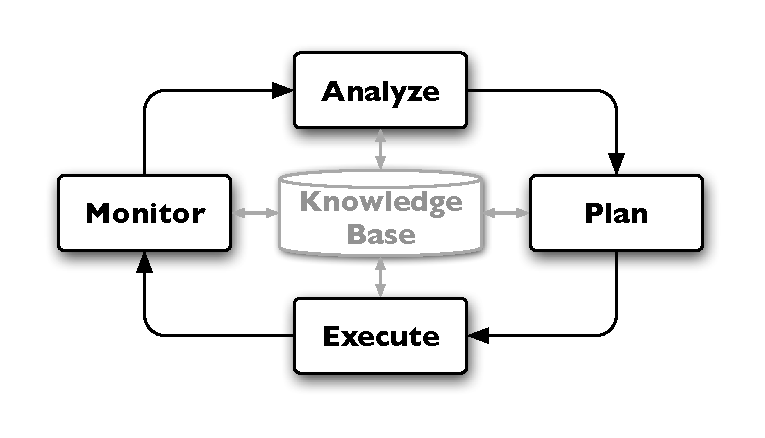
\includegraphics[width=\columnwidth]{mape.eps}
	\caption{General MAPE control loop}
	\label{fig:MAPE}
\end{figure}

In order for the system to analyze and interact with its environment there is a need for some type of input and output. The input of environmental information is transferred by so called \textit{sensors} and the output to enact the planned actions are sent using \textit{effectors}. For the framework to be useful it is not necessary however that these parts, nor the MAPE tasks, are computerized. It is possible to have human interaction integrated into the system description.

\subsection{Problem}
The current workflow for managing online marketing campaigns starts with the creation of advertising material by the advertiser. Once the ads have been run, their impact is analyzed and based on these results, material can be created, adapted or removed from circulation to better suit the goals of the organization. For example, ads with a low click rate need to either be removed completely or modified in some way in order to increase their efficiency, whereas an ad that performs very well most likely is left as is and used as inspiration for new ads.

There is a high cost for this repetitive manual labor in terms of both time and money, since the data must be analyzed over and over again. This may not be a problem for small sets of data, but it becomes increasingly hard to maintain as the number of campaigns and ad properties grow over time. Company A, for example, has hundreds of campaigns running at once and the amount of historical data grows quickly which means that managing this data becomes cumbersome.

The problem is thus one of managing historical advertisement data and applying that data to future decisions in order to optimize the future overall click rate of the organization's ads. In business intelligence terms, the goal is therefore to apply an analytical tool to the stored data in order to provide decision makers with knowledge that can be enacted upon.

\subsection{Solution}
The basic requirement of a system which could solve the previously stated problem is that it should be able to analyze existing campaigns and their metrics and use this as a basis for suggesting new ads to the operator\footnote{As the word \emph{user} is typically used to refer to a person interacting with either the web site that is being marketed or the web site on which the advertisement is shown, we will use the word \emph{operator} when discussing a person interacting with the system that is described in this paper to avoid confusion.} based on the estimated performance.

The proposed solution is to apply the principles of automation described in the MAPE framework to the context of marketing. Monitoring is thus the collection of metrics for online advertisement. To optimize these metrics, the gathered information is analyzed and this analysis forms the basis for the planning of future campaigns to run. Once the plans are completed, they are presented to the operator who can execute them, after which new metrics are gathered and so on.

It is already common for monitoring to be automated, either using custom software or services such as Google Analytics\footnote{http://www.google.com/analytics/}, whereas the other parts of the process are performed manually. It is infeasible to fully automate the whole process, due to for example the creative side of advertisement including creating new photos and writing new texts. There are however certain areas that can be automated and this paper will focus on automated analysis and planning of online marketing campaigns, shown in Figure \ref{fig:MAPEMarketing}.

\begin{figure}[htb] \centering 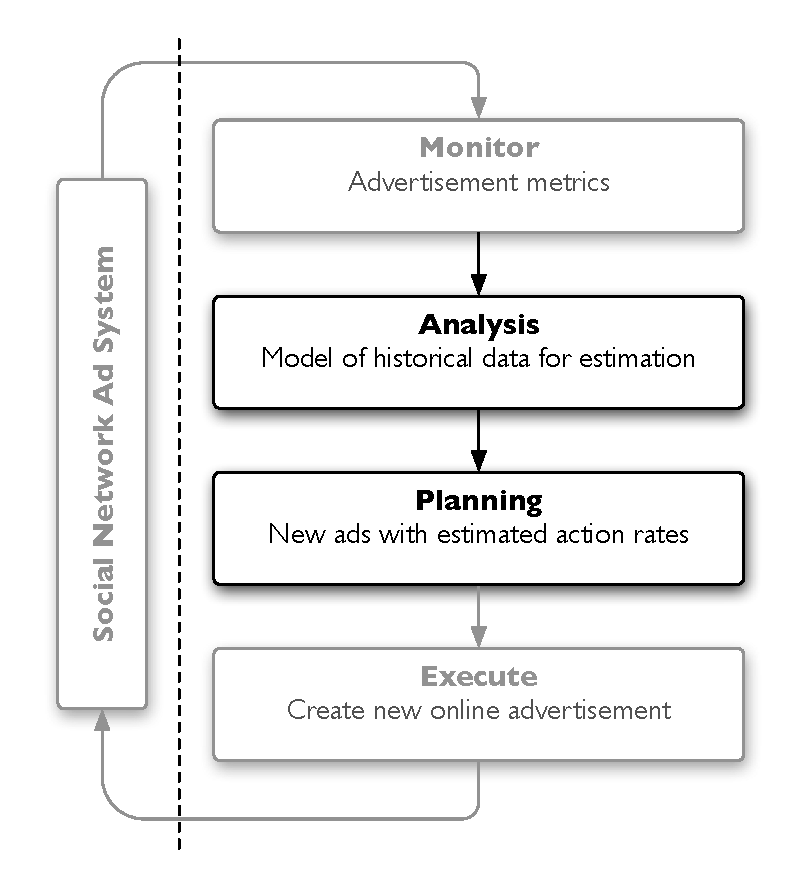
\includegraphics[width=0.96\columnwidth]{mape-marketing.eps}
	\caption{Online marketing automation system in control loop}
	\label{fig:MAPEMarketing}
\end{figure}

A system to automate this process requires monitored data as input, which in this context equals historical data of campaigns and their metrics as mentioned previously. This data is then analyzed and modeled so that an estimated action rate can be estimated based on the properties of the ad. Because Company A only targets their ads based on gender, between which there are significant differences in how the ads are designed, targeting will be handled by dividing the full data set into subsets based on the target and then apply the solution to each such subset independently.

Based on this model, the system will generate suggestions for new campaigns as well as recommend actions to be taken by the operator to optimize the overall average action rate of existing ads.

\subsection{Scope}
Using the MAPE framework in Figure \ref{fig:MAPE}, only the analysis and planning tasks are considered part of this paper, whereas monitoring and execution are out of scope. The latter two are of course relevant in the implementation of the system, but neither will be covered as a research topic. In this context, this means for example that the feature of integrating this system with marketing services to automatically add new ads and campaigns will not be a part of the final system.

Furthermore, the data set will include attributes whose values are free text and images, however text mining and image recognition are beyond the scope of this project.

The model of the marketing domain purposefully excluded references to costs and budgets. Though the economy of marketing is of great interest to the advertiser, we have assumed that the most important part of the process is to optimize the number of actions (which in our specific case is the same as clicks, as mentioned previously). This assumption was approved by our industrial partner.

On the topic of costs and budgets, it is also necessary to mention that due to the costs of running advertisement, there was a limitation on the types of experiments we could perform. Thus large scale live testing of the system is not included in the scope of this thesis.

Finally, targeting will only be covered briefly and for the specific case of Company A. A general solution for managing different types of targeting and how they influence estimations is thus not a part of this thesis.

\subsection{Thesis outline}
This section has provided an overview of the domain, a description of the problem as well as a brief outline of the suggested solution. It has also defined the scope of this thesis.

Section \ref{ch:Foundations} will cover research foundations for this paper, mostly in the area of knowledge discovery and data mining. This is followed by section \ref{ch:RelatedWorks} which summarizes research efforts related to the field of online marketing.

Section \ref{ch:Method} describes the method used to develop the solution, the research questions that defined the focus of our research as well as an explanation of the data used to experiment on.

Section \ref{ch:Solution} then answers the research questions and the solution is developed and explained based on those results.

Finally, section \ref{ch:Conclusion} gives a summary of the results presented in this paper, discussion on risks and constraints as well as suggestions for future work.

\section{Foundations}
\label{ch:Foundations}
% Knowledge Discovery
The problem as well as solution described in the introduction show there is a need to have a software system which can parse and analyze large sets of data. To facilitate this, a number of high-level descriptions of frameworks for knowledge discovery in databases exist \citep{Fayyad1996, Frawley1992} and they exhibit a number of commonalities. These include the importance of having a knowledgeable human operator guiding the process in terms of supplying domain knowledge to the system formulating the goal of the knowledge discovery; feeding discovered knowledge back into the system; and the identification and application of a discovery method, or more specifically the data mining algorithms. Because the solution is a knowledge discovery system, it is important that it too has these same characteristics.

% Data mining
In data mining, the input to a system can be described using the terms \emph{concepts}, \emph{instances} and \emph{attributes}, where concept is the actual result of the mining, i.e. what we want to be learned; an instance is one single example of data to be mined and can be compared to a row in a database; and attribute is a property of an instance, which in the database analogy is a column \citep{Witten2011}. This analogy is useful since it is directly applicable to the structured internal data the system uses as input, as defined in the introduction.

Kantardzic gives a top-down explanation of data mining, where the learning methods can be divided into two classes; supervised learning and unsupervised learning \cite{Kantardzic2011}. In the first case, the learning is based on existing instances and the known values of a dependent variable for each such instance, whereas unsupervised learning has no knowledge of such a dependent variable and thus is only concerned with identifying structure in the input data. The structured input data will have such a dependent variable, or at least it can be calculated from existing variables (e.g. the number of clicks divided by the number of impressions gives the average click rate of a campaign). This means that we are dealing with supervised learning.

Within supervised learning there are a number of different types of learning tasks, and Kantardzic goes on to describe classification as the most common such task \cite{Kantardzic2011}. The purpose of a classification algorithm is to categorize an instance into a predefined class, based on existing instances that are already classified. This is not directly applicable to the marketing data, but Witten et al. describe a special case of classifiers where the outcome is a real number instead of a class \citep{Witten2011}. This type of classification is referred to as numeric prediction or numeric classification, and the technique will be evaluated for use in estimation of action rates for new campaigns. In the case of marketing, another possibility is to use classifiers which provide probabilities of class association as well. By looking at each impression as a trial, each ad has a probability of belonging to the class of being clicked.

\section{Related work}
\label{ch:RelatedWorks}
There have been some research in methods for estimating the performance of online advertisement, though no such research seems to exist for social network advertisement specifically. We begin by looking at related work for ad performance estimation in search advertisement, followed by techniques for improving, though not estimating, performance. Finally we describe research concerning how users experience ads and potential problems caused by fake traffic.

Richardson et al. describe a model for predicting the click-through rates of ads given a set of properties in the context of search engine advertisement \cite{Richardson2007}. For the estimation, the authors use logistic regression on a large number of ad features (e.g. number of characters in text and segments in URL). This approach is chosen in the paper because logistic regression provides a probability for class association, and a click probability is the goal. There is however no further discussion or experimentation to elicit why this choice is more appropriate than for example numeric classifiers. The results are nevertheless promising in regard to the predictive powers of logistic regression and as such it will be evaluated as a potential estimation model in this paper.

Another paper on predicting click-through rate (CTR) use a cluster analysis approach \cite{Regelson2006}. In order to estimate the CTR of a search term, a number of related search terms with known performance are identified and used as a basis for the prediction. Though the method performs well, it is tightly bound to the field of search engine advertisement. The same can be said for \cite{Richardson2007}, which for example utilizes correlation between search terms to improve estimates. Because the concept of search terms does not exist in social networking advertisement, neither approach is directly applicable.

Automation in marketing is not a completely novel idea. Joshi and Motwani present a technique for automatically finding related keywords for broader targeting of ads by creating a graph of search terms based on the domain knowledge contained in search engines \cite{Joshi2006}. Continuation of that work is that of Thomaidou and Vazirgiannis, where keywords are also extracted from the landing page to further improve the results \cite{Thomaidou2011}. Both approaches are however only relevant for contextual and search engine advertisement as they use data exclusive to the respective advertisement class.

Marketing in the context of social media has also gained interest in the academic community. Yang et al. propose a technique for identifying subgroups of users in social networks based on their interactions and then use that information to create targeted advertising \cite{Yang2006}. The results could very well be applied in parallel to the results of this thesis in order to better target ads, however it does not deal with ad performance in any way.

Research has also shown that using targeted advertisement is effective given that the ad is not experienced as being obtrusive, though obtrusive ads that are not targeted (i.e. non-contextual) also increase performance \citep{Goldfarb2011}. Another study presented results that suggest that users on social networks generally tend to not consciously take notice of advertisement and, perhaps of this meaning that ads are not considered to be obtrusive, they do not have any negative feelings toward the existence of advertising \citep{Hadija2012}. By automating the process of estimating ad performance, these properties for ad management are expected to be implicitly handled by the model, since properties that make users experience the ad as obtrusive or unnoticeable will perform worse and thus those results will impact future estimates.

In online advertisement there have been problems of so called click-spam or click-fraud, meaning that the number of clicks on ads is increased in a fraudulent manner, for example using bots. Dave et al. provide a methodology to measure click-spam in their networks as well as a study of the severity of the problem on different classes of networks \cite{Dave2012}. Their results show that established search advertising on for example Google and Bing is fairly accurate in their filtering of click-spam, whereas the problem is greater for contextual and social advertisement, and severe for mobile advertisement. A related paper describes a methodology for advertisers to evaluate the quality of click traffic and use this to assess the difference in quality between bulk traffic vendors and established pay-per-click networks \cite{Zhang2011}. It may be of importance to be aware of these issues as they could carry some impact on the research, however managing traffic quality and click-spam is not in the scope of this paper.

In conclusion, though predicting performance of ads has seen some limited research, the area of social networking advertisement is largely unexplored, especially in terms of performance prediction.

\section{Method}
\label{ch:Method}
This section describes the process that was used to identify a solution to the problem described in the introduction. The first step of the process was a literature review to identify existing research in this area and examine the foundations. Simultaneously, meetings were held with marketing experts from Company A to define the domain in which to apply the results of the project.

The next step was obtaining a sample of real world marketing data for analysis and experimentation. This process began with manual analysis and then formalized experiments to confirm the idea that the data could be modeled in order to provide better-than-random estimates. Once that had been established, the appropriate choice of classifier was evaluated.

Once the modeling and estimation part of the research was concluded, the question of planning was approached. This dealt with defining how an operator should select ads from the system's suggestions and analyzing if ad performance declines over time in order to suggest when an existing ad has run its course.

The problems described above were formulated as research questions that are covered in more detail in section \ref{sec:ResearchQuestions}.

Finally the pieces were put together in the form of a software application with an easy-to-use graphical user interface.

The last subsection in this section describes the sample data provided by Company A to help the reader understand the structure of a typical data set.

\subsection{Research questions}
\label{sec:ResearchQuestions}
In formulating the research questions, the definitions provided by \cite{Shaw2002} were used in order to provide clear goals for what the thesis should provide.

\textit{\textbf{RQ 1.} How to automate the creation and estimation of good ads in online marketing?}
The main research question for this thesis is the identification of a method of development that can be used in organizations to support decisions in online marketing. The solution presented is a procedure that is applicable to online advertisers.

Because this question is very broad, the validation step consisted of dividing the question into four sub-questions and validating them each in turn.

\textit{\textbf{RQ 1.1.} Do ad properties have differing impact on performance?}
It would be reasonable to assume that different properties of an ad may have different impact on the user it is shown to in terms of likelihood of him or her taking an action, however the size of those differences are harder to hypothesize about. This is an important first question in order to get an indication of how, if at all, properties relate to the click rate.

To answer the question, a controlled experiment was defined were ad properties were carefully selected by domain experts and then tested in a real world environment. From the resulting metrics, the correlation between properties and performance was calculated and analyzed.

\textit{\textbf{RQ 1.2.} How well do classifiers perform in estimating click rates?}
The first step is to identify whether or not a numerical classifier can, based on historical data, adequately estimate the action rate of previously unseen ads. It is thus a matter of evaluating the performance of existing algorithms.

To provide an answer to the question an experiment was defined, where the success rate of a regression model was compared to those of random values from statistical distributions, one normally distributed and one uniform distribution with the same minimum and maximum values as the data set, as well as comparing success rates of different classifiers to each other. The results answer both how well classifiers perform in relation to simpler models, and if they perform better, which classifier is most suited for the task.

\textit{\textbf{RQ 1.3.} Which ad selection strategy provides the highest average click rate?}
It is unlikely that a classifier would correctly estimate future ad performance every time. To potentially minimize the impact of bad estimations, multiple suggested ads could be selected by the operator and run together in order to improve the average action rate.

To evaluate this six different strategies were tested, where one, two and three suggested ads were selected based on their estimated performance after which the average real performance both with and without weighting based on the estimates were calculated. The results were then analyzed to identify the appropriate strategy to use.

\textit{\textbf{RQ 1.4.} How does time affect the performance of ads?}
A marketing executive suggested that the performance of ads declines over time. To evaluate the correctness of this statement, data was gathered over a period of two weeks where the same ads were run continuously and then analyzed. Depending on the answer, the final solution would possibly have to account for such a decline in estimating the future performance of existing ads.
\newpage
\subsection{Data set}
The main data set used for analysis and experiments was provided by Company A and consisted of ads run in the Polish market between July 17\superscript{th} and August 17\superscript{th} 2012. The set contained 959 instances of ads run on Facebook in the mentioned time interval. All ads had however not been run for the whole time.

There were a total of eight (8) unique titles, but six of those where almost equal with only difference being the city they referred to. The body texts had three (3) distinct values, and by counting the titles referring to a city as a single title, every title was used exclusively together with a single body text so that only three possible title/body combinations existed. A total of eleven (11) unique images were used, out of which five (5) were used when targeting both genders and each gender having three (3) exclusive images. Figure \ref{fig:AdLayout} shows the layout used by Facebook, with the title above the image and the body text to the right of the image. This layout is fixed and cannot be modified by the operator, who can only set the individual properties for the ad (and of course also targeting properties).

\begin{figure}[htb]
	\centering
	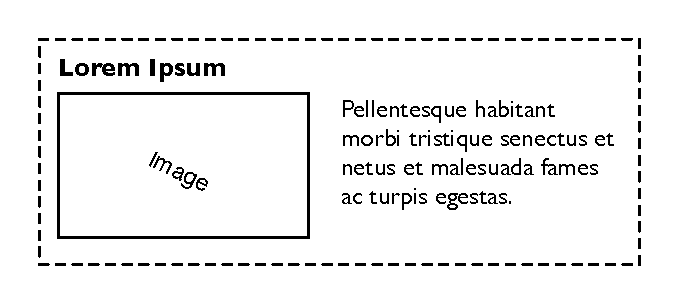
\includegraphics[width=\columnwidth]{ad-layout.eps}
	\caption{Layout for ad presentation}
	\label{fig:AdLayout}
\end{figure}

The average number of impressions for each ad in the data set was 143875.17 and the average number of clicks was 32.96, both values with two decimals of precision. By dividing the clicks with the impressions we get an average click-through rate of about 0.0229\%.

Over the course of this project, Company A made some changes to their marketing strategy. The most noticeable difference was the removal of distinct age groups for targeting, which left gender as the only targeting property. To still be able to use the data set, the metrics of campaigns that only differed in the targeted age group were aggregated. This aggregation reduced the number of unique instances to 64. Other changes to the strategy included using the same title on all ads and changing the regions in which marketing took place, however the data set was not adapted to reflect these changes since those changes could not be simulated using for example aggregation.

\subsubsection{Tagging data}
An early idea on how to modify the data to provide more insights for the operator was to apply tags to the images and texts. Tags are a set of words that describe an object, so that similarities can be discerned more easily by a computer system. There were however two main problems with this method. First of all, there is the question of subjectivity. This is especially a problem for pictures, whose information content is highly unstructured making the set of possible attributes that are important hard to define. As an example, imagine an ad with a picture of a girl sitting in a coffee shop. A user's likelihood of clicking the ad may either increase or decrease depending on the looks of the girl, the lighting in the room, what beverage the girl is drinking, whether there are other people around or not, etcetera. The subjectivity involved (who decides whether a person is good-looking or not?) and the nearly unlimited possible attributes were the main reasons for ruling out image tagging.

For texts it is possible to remove a lot of the problems with image tagging by only focusing on the actual words that appear. This does however lead to a new problem, which would also have affected image tagging if it was applied despite the concerns raised. Consider the case of two high performing ads, one with the tags "beach" and "volleyball", the other one with tags "snow" and "skiing". Because a classifier is not aware of the context, it is feasible that it would estimate an ad focusing on for example "beach" and "snow" to have a very high click rate, though this is in reality unlikely to be true. Also considering that tagging could easily introduce thousands or millions of possible combinations to be estimated, this would mean the operator would need to do a lot of extra work in ruling out these misguided suggestions and the whole purpose of the system would be defeated.

\subsubsection{Statistical distribution}
A visual analysis of a graph of the click rates hinted of a normal distribution. To judge whether this was the case, the extended Shapiro-Wilks normality test \citep{Royston1982} as implemented in R\footnote{http://www.r-project.org/} was used. Ads that had not received any clicks were considered to be outliers and removed from the sampling to not skew the results. This turned out to only affect a single ad.

A significance level, \(\alpha\), of 0.05 was chosen for the null hypothesis \(H_0\), which would mean the data is normal. The test returned the test statistic \(W = 0.9654\) and a p-value of 0.07339. Since \(0.07339 > \alpha\), we cannot reject \(H_0\) and therefore we assume a normal distribution of the data set.

When no specification is made in regard to which data set was used for a specific experiment, it is implied that the results are based on the part of the aggregated data set which targeted women. Though all experiments have been run on both subsets, we have chosen to only give the results of one set as long as the conclusions of the results are the same.

\section{Solution}
\label{ch:Solution}
The proposed solution to the problem is to automate the creation of good ads for online marketing using a software system. Figure \ref{fig:SWArchitecture} gives an overview of the architecture for such a system. The main components include a data manager for interacting with the knowledge base, an estimator that based on historical data can estimate the performance of new ads and an ad factory that can provide new ads with unknown performance to, for example, an estimator.

\begin{figure}[htb]
	\centering
	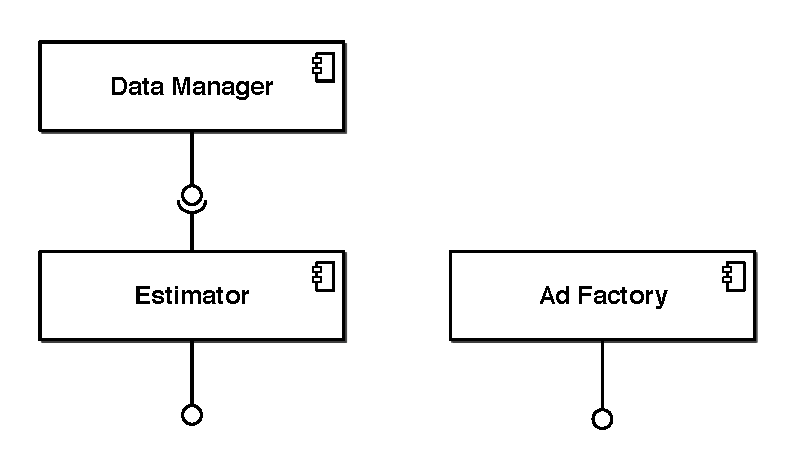
\includegraphics[width=\columnwidth]{sw-architecture.eps}
	\caption{Component diagram of software solution}
	\label{fig:SWArchitecture}
\end{figure}

In order to answer the research questions, the estimator, which is the central part of the system, must be evaluated. By having an evaluator which controls the interfaces to and from the estimator as in Figure \ref{fig:SWEvaluator}, we can create a number of different evaluators to test different aspects of the estimation.

\begin{figure}[htb]
	\centering
	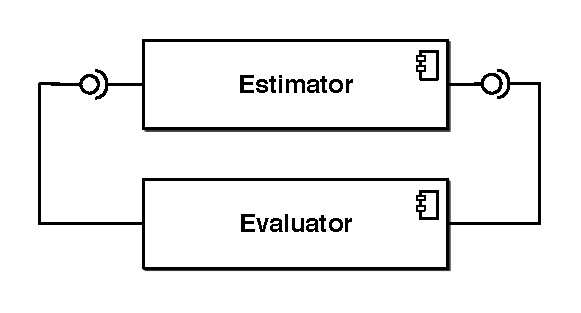
\includegraphics[width=0.65\columnwidth]{sw-evaluator.eps}
	\caption{Component diagram of system evaluation}
	\label{fig:SWEvaluator}
\end{figure}

Because the evaluator controls the input to the evaluator component, ads whose performance is known can be input to the application and its output compared to the actual values. This comparison is useful for gaining insight into how well the estimates reflect reality. More specifically, by repeating such an experiment many times but change the data set used, we get a reliable indicator of how well an estimator performs, namely the percentage of trials for which the estimate was reasonably close to the actual value. This of course requires a definition of what reasonably close means, something which will be covered in section \ref{ssec:Classifier}. These indicator values can also be compared for different estimators to identify which is the most accurate one, which is also done in the mentioned section.

\begin{figure}[htb]
	\centering
	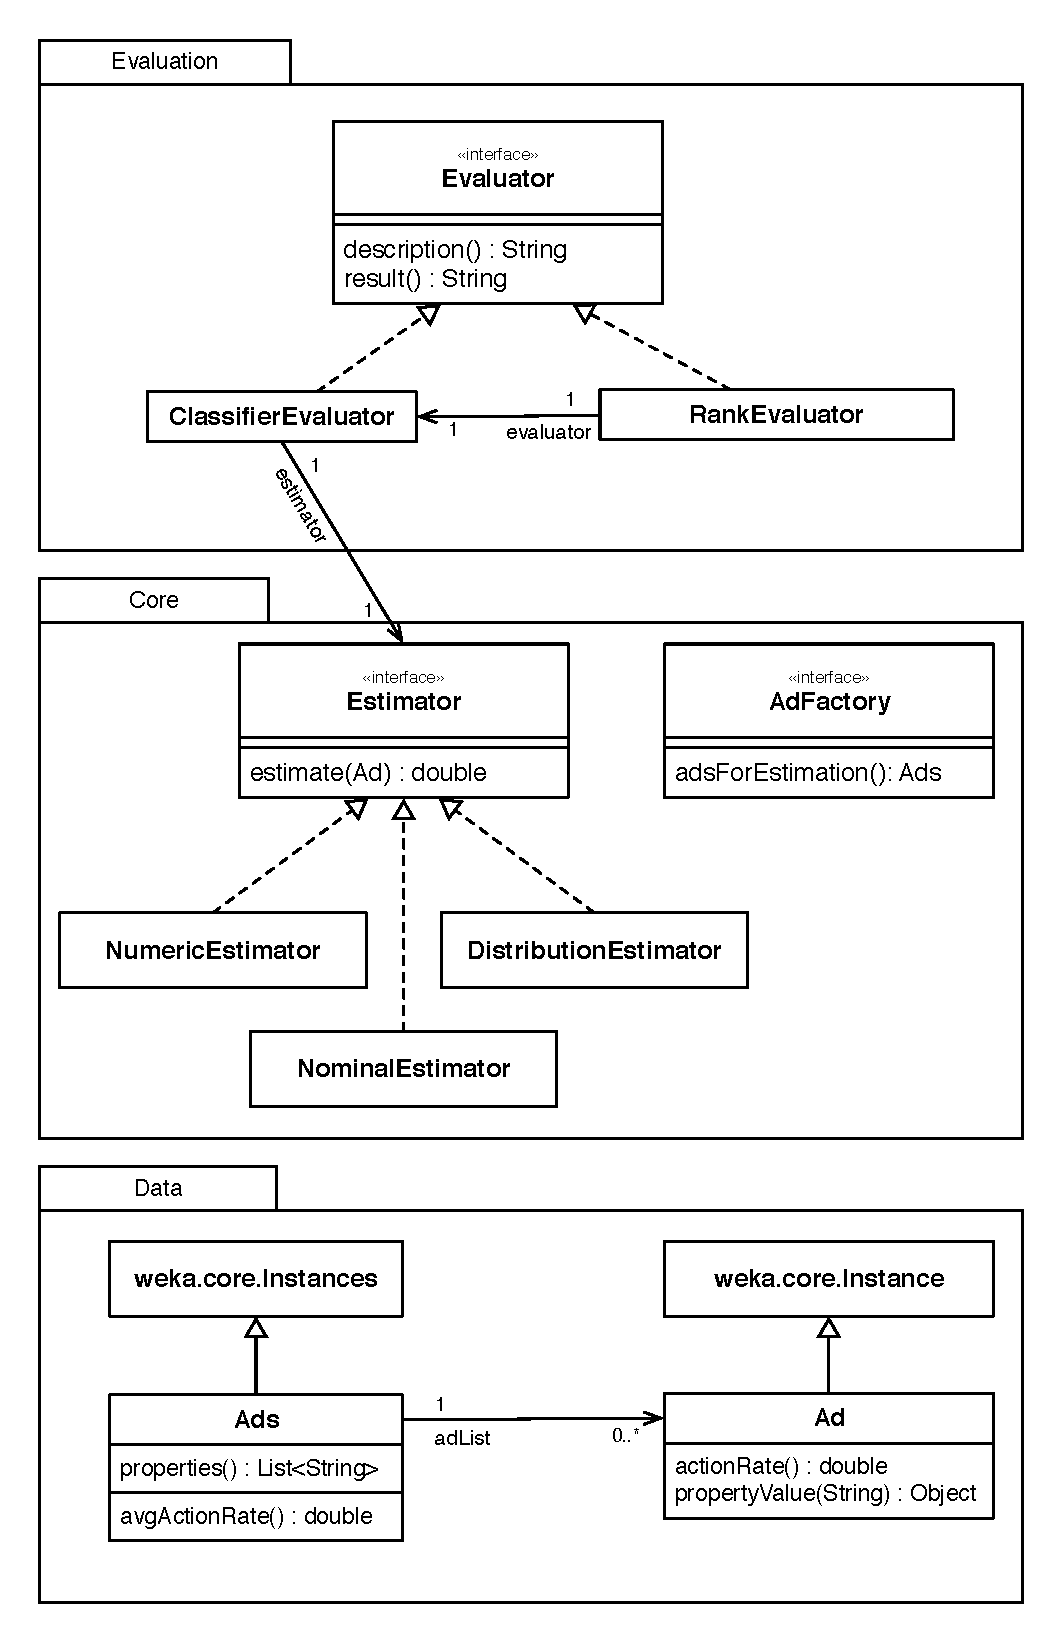
\includegraphics[width=\columnwidth]{class-diagram.eps}
	\caption{Class diagram of system}
	\label{fig:ClassDiagram}
\end{figure}

It is important to know that the developed system takes advantage of the Weka library \citep{Garner1995} by using its classes for modeling the data sets and its implementations of classifiers. It also uses the Colt library\footnote{http://acs.lbl.gov/software/colt/} for dealing with statistical distributions.

The Data package defines the main classes that model the data. The main purpose of \textit{Ads} is to manage a list of single \textit{Ad} objects that all store the same type of information. It is data from these classes that is used by the logic in the Core package.

The main interface in Core is the \textit{Estimator}, whose purpose it is to predict the performance of an ad whose performance is not known. The different realizations of this interface represents different methods of prediction, with the \textit{NumericEstimator} utilizing numeric classifiers, the \textit{NominalEstimator} returns the probability that the ad belongs to the class of clicked ads, and the \textit{DistributionEstimator} uses statistical distributions to randomly assign a prediction.

An AdFactory is basically a provider of ads which do not have an estimated action rate. The source of these ads can be for example combinations of ad properties for which no metrics exist, or suggestions input by an operator. The realization of this interface is closely tied to the environment in which the system will exist.

The final package is Evaluation, whose only interface is \textit{Evaluator}. The requirements of its implementations are to provide a textual description of what it does and of its results, which were used in the validation of this system. The \textit{ClassifierEvaluator} creates its results by instantiating an Estimator with known data, and can then compare the estimates to some known reference values. One such example was described in the beginning of the section, where the action rates of the ads in the AdFactory are saved and compared to the estimated results.

The \textit{RankEvaluator} in turn does not require an Estimator directly, but rather utilizes the results of the ClassifierEvaluator to establish how well classifiers perform for different selection strategies, as described in RQ 1.3.

This overview of components and classes has explained how the software was designed. The following subsections will first suggest how to create the knowledge base required by the system, followed by descriptions of the validation experiments and their results.

\subsection{Knowledge base}
The data manager was mentioned as the component which interacts with the knowledge base. The knowledge base contains all historical data used by the system and must thus not only be able to provide data, but also be updatable. The actual contents of the knowledge base should be limited to only the data which is used by the other components to conserve space, unless that specification of what is useful and not is likely to change.

An efficient way of storing the structured data that we are dealing with is a database, and was also the solution used in our implementation. By storing only the necessary data in a database and updating it whenever new monitored metrics are available, not only is the data manager's task simplified but the data can also be queried from outside the system which avoids lock-in of data, something that could be a problem for some organizations.

\subsection{Impact of properties}
To show whether different properties carry different weight in regard to how well an ad performs was an important first step in order to get an indication of the potential merits of modeling the data. For example, if an ad consists of an image and a text, are the choices of image and text equally important in the search of a high-performing ad or does one carry a stronger influence on the final result than the other? Or even more importantly, if the properties carry no correlation to the click-rate, that would imply performance has nothing to do with the ad properties defined by the advertiser.

Domain experts from two geographical markets, Brazil and Argentina, were asked to choose three ads that they had previously run in their market which they identified as representative of high, average and low performance respectively. The three performance levels were chosen to get a baseline performance as well as more extreme values in both directions. The selection was done for men and women separately, so a total of six ads were selected for each region. It is important to note that these were existing ads, so while they performed differently the choice of for example the lowest performing ad was not a manufactured ad whose purpose was to perform badly (e.g. by selecting an offensive image). Finally combinations of the three images and three texts within each region and gender were formed and put online.

The budget for the experiment was 720 USD, or 20 USD per ad. For Brazil this generated an average of 179124 impressions and 77 clicks, and for Argentina those numbers were 382791 and 126 respectively. Once the budget was spent, the results were collected and the correlation coefficient was calculated for each property and the resulting click rate. Each region's data set was also split by gender to see differences between target groups. Finally, the data was gathered and the correlation was calculated. We used the Pearson coefficient of correlation \cite{Milton2002}, which is defined as

\begin{equation}
	\rho = \frac{Cov(X, Y)}{\sqrt{(Var X)(Var Y)}}
\end{equation}

In our case, the random variables \(X\) and \(Y\) represent the choice of value for a given property and the click rate respectively. Because the covariance and variance are unknown they have to be estimated based on the sample.

\begin{equation}
	\hat{\rho} = \frac{\widehat{Cov(X, Y)}}{\sqrt{(\widehat{Var X})(\widehat{Var Y})}} = \frac{ \sum_{i=1}^{n} (X_i - \bar{X})(Y_i - \bar{Y}) }{ \sqrt{ (\sum_{i=1}^{n} (X_i - \bar{X})^2) (\sum_{i=1}^{n} (Y_i - \bar{Y})^2) } }
\end{equation}

Because we are only interested in how big the impact is of different properties and not if said impact is positive or negative, it is the magnitude of the correlation which is important and not the direction. Since \(-1 \leq \hat{\rho} \leq 1 \), we therefore used the absolute value \(|\hat{\rho}|\) for comparison. As an example, even if the correlation for a property is near -1, the conclusion is still that it has a large impact on the performance. In other words, the interpretation of \(|\hat{\rho}|\) is that if it is 1 there is an exact linear correlation between the two random variables whereas 0 means there is no linear correlation at all. The results of the experiment are presented in Figure \ref{fig:PropertyImpact}.

\begin{figure}[htbp]
\begin{center}
	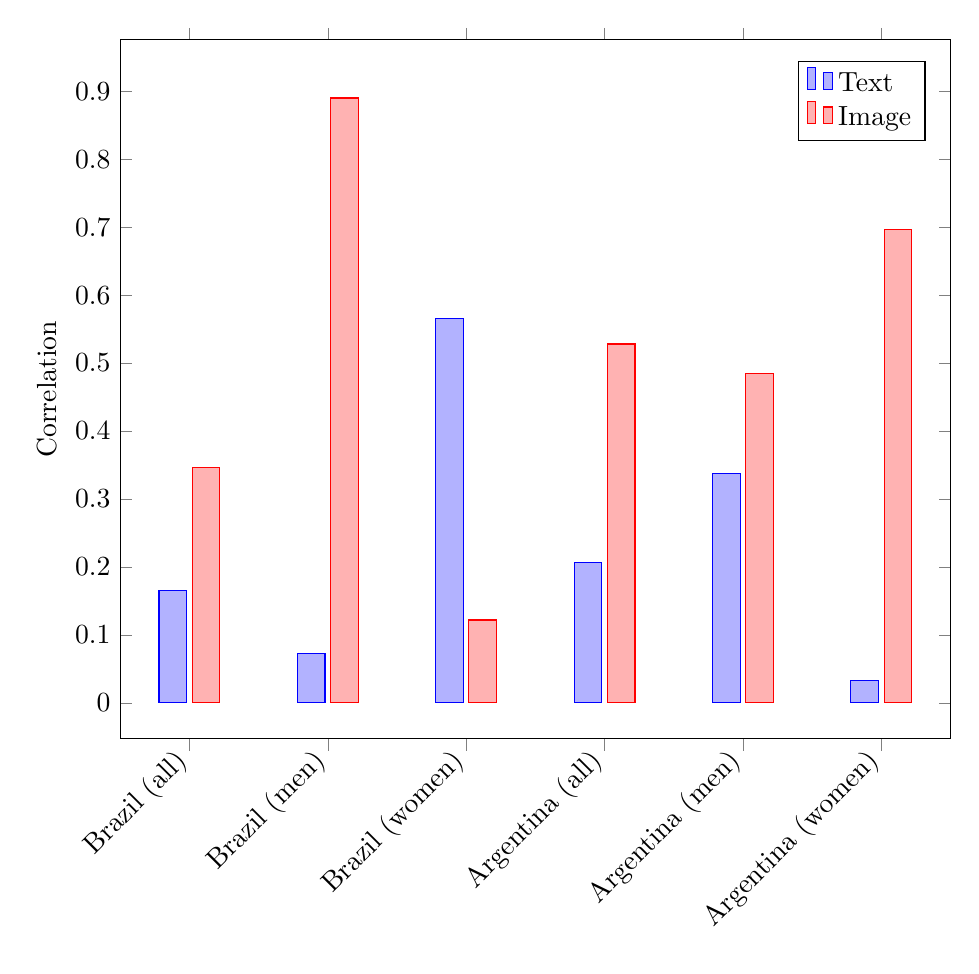
\begin{tikzpicture}
	\begin{axis}[
	    ylabel={Correlation},
	    ybar,
		legend style={
			cells={anchor=east},
			legend pos=north east,
		},
		legend cell align=left,
		width=\linewidth,
		symbolic x coords={Brazil (all),Brazil (men),Brazil (women), Argentina (all), Argentina (men), Argentina (women)},
		xtick=data,
		x tick label style={rotate=45,anchor=east},
	]
	\addplot coordinates {(Brazil (all), 0.165) (Brazil (men), 0.073) (Brazil (women), 0.566) (Argentina (all), 0.206) (Argentina (men), 0.338) (Argentina (women), 0.033)};
	\addplot coordinates {(Brazil (all), 0.347) (Brazil (men), 0.89) (Brazil (women), 0.122) (Argentina (all), 0.528) (Argentina (men), 0.485) (Argentina (women), 0.697)};

	\legend{Text, Image}
	\end{axis}
	\end{tikzpicture}

	\caption{Impact of text and image in ad performance}
	\label{fig:PropertyImpact}
\end{center}
\end{figure}

The results clearly show that the impact of the choice of image is larger than that of the choice of text. Most notable are perhaps the correlation values for men in Brazil and women in Argentina where the image is of utmost importance, as well as the result that women in Brazil are the only group where the text has a higher impact than the image.

Because of the large differences, the results were discussed with one of the domain experts involved in the ad selection. Overall he considered the results to be in line with his expectations, even though the high correlation between text and CTR for women in Brazil and men in Argentina were slightly higher than he would have guessed. A suggested reason for this was that the gender of the domain expert in each region was the opposite of the gender for which the texts were more important than expected (i.e. a heterosexual man is better at selecting high performing images of women and vice versa). Because of this, further experiments will be made at Company A to compare image selection between men and women, however those experiments will not be part of this paper.

The results nonetheless provide an answer to RQ 1.1, as there is a noticeable difference in the impact of the two properties used in this example.

\subsection{Rate estimation}
The working hypothesis was that a numerical classifier could estimate the action rate of new ads sufficiently well. By manual experimentation with the data set in the Weka workbench, a support vector regression algorithm called Sequential Minimal Optimization (SMO) was identified as a good candidate for further experimentation.

The experiment was designed as follows. Initially, the data set was randomly split into two separate, non-overlapping sets called training and validation. The training set was then used to create the regression model, after which the action rate of the validation instances was estimated. For each such estimate, an estimate was considered successful if the following inequality held true.

\[
	c_i - \epsilon \leq \hat{c}_i \leq c_i + \epsilon
\]

\(c_i\) is the actual action rate for ad i in the validation set and \(\hat{c}_i\) is the estimated value. The tolerance limit is defined as \(\epsilon = k*\bar{c}\), where \(k\) is a constant between 0 and 1. This process was repeated 5000 times and both the total number of estimations as well as the number of successful estimations were counted. From this a success percentage was calculated for different values of \(k\).

For comparison, the same process was also applied with two simple statistical models of the training set. The simplest model was defining a uniform distribution between the minimum and maximum values in the data set, and the slightly more advanced model assumed a normal distribution. The latter was used due to our previous assumption that the data is in fact normally distributed. The estimations from these models were then made by drawing a random value from the distribution. Table \ref{tbl:EstimationSuccess} and Figure \ref{fig:EstimationSuccess} show the results of the experiment for all three models.

\begin{table}[htbp]
\begin{center}
	\begin{tabular}{ l | r r r r }
		\hline
		\textbf{Method} & \textbf{k=0.01} & \textbf{k=0.05} & \textbf{k=0.10} & \textbf{k=0.20} \\
		\hline
		Uniform & 1.51\% & 7.41\% & 14.32\% & 29.74\% \\
		Normal & 2.55\% & 12.99\% & 25.72\% & 48.50\% \\
		SMO & 1.84\% & 14.66\% & 34.19\% & 72.96\% \\
		\hline
	\end{tabular}
	\caption{Estimation success percentage over 5000 rounds}
	\label{tbl:EstimationSuccess}
\end{center}
\end{table}

\begin{figure}[htbp]
\begin{center}
	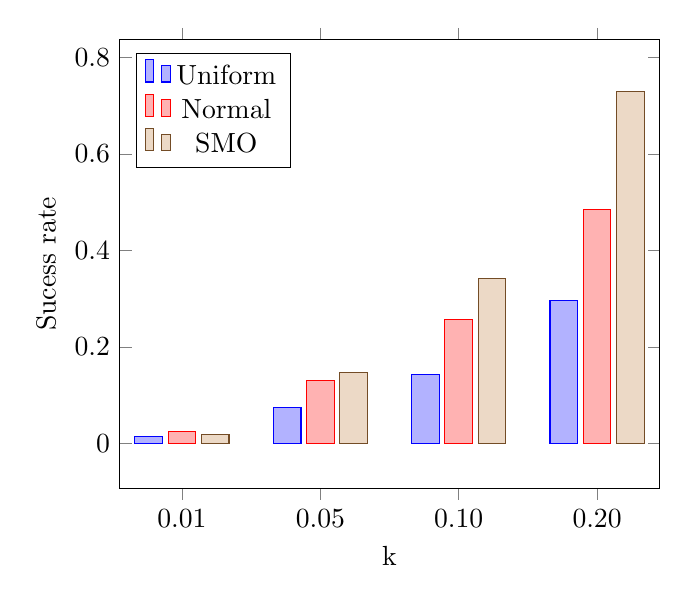
\begin{tikzpicture} \begin{axis}[
	    ybar,
	    enlargelimits=0.15,
	    legend pos=north west,
	    ylabel={Sucess rate},
	    xlabel={k},
	    symbolic x coords={0.01,0.05,0.10,0.20},
	    xtick=data,
	    ]
	\addplot coordinates {(0.01, 0.01505) (0.05, 0.07405) (0.10, 0.14315) (0.20, 0.2974)};
	\addplot coordinates {(0.01, 0.0255) (0.05, 0.1299) (0.10, 0.2572) (0.20, 0.4850)};
	\addplot coordinates {(0.01, 0.0184) (0.05, 0.1466) (0.10, 0.3419) (0.20, 0.72955)};
	\legend{Uniform,Normal,SMO}
	\end{axis}
	\end{tikzpicture}
	\caption{Bar chart of Table \ref{tbl:EstimationSuccess}}
	\label{fig:EstimationSuccess}
\end{center}
\end{figure}

The value of \(k\) defines how large the interval of success is, and thus if \(k\) is increased enough, success is always guaranteed no matter the estimate. Figure \ref{fig:KImpact} shows the size of the success spans for the values used in the previously mentioned experiment, with estimate \(\hat{c} = 0.00025\) and mean \(\bar{c} = 0.00020\).

\begin{figure}[htb] \centering
	\begin{tikzpicture} \begin{axis}[
	    axis y line=left,
	    axis x line=bottom,
	    ylabel={k},
	    width=\linewidth,
	    height=0.45\linewidth,
	    xtick={0,0.00010,0.00020,0.00030},
	    xticklabels={$0$,$0.00010$,$0.00020$,$0.00030$},
	    xmin=0.0,
	    xmax=0.00030,
	    ymax=5,
	    ytick={0,1,2,3,4},
	    yticklabels={$0$,$0.01$,$0.05$,$0.10$,$0.20$},
	]

	\addplot coordinates {(0.00025, 0) };
	\addplot+[mark={|}, line width=1pt] coordinates {(0.000248, 1) (0.000252, 1) };
	\addplot+[mark={|}, line width=1pt] coordinates {(0.00024, 2) (0.00026, 2) };
	\addplot+[mark={|}, line width=1pt] coordinates {(0.00023, 3) (0.00027, 3) };
	\addplot+[mark={|}, line width=1pt] coordinates {(0.00021, 4) (0.00029, 4) };

	\end{axis}
	\end{tikzpicture}

	\caption{Impact of \textit{k}-values on success intervals}
	\label{fig:KImpact}
\end{figure}

As \(k\) increases it becomes clear that the regression model is noticeably better than the statistical distributions. At \(k \approx 0.036\) the regression model and the normal distribution perform equally well, and as \(k\) increases the regression model becomes increasingly better in relation to the distribution, which answers RQ 1.2. Additional experiments also revealed that the regression model reached a 50\% success rate at \(k \approx 0.135\).

\subsection{Choice of classifier}
\label{ssec:Classifier}
Even though the SMO algorithm performed well for estimation, the choice of algorithm was mainly an educated guess. As  different classifiers tend to be best suited for different situations, the estimation experiment was revisited to identify the best choice of classifier for this purpose. The only difference was that for this experiment the statistical distributions were replaced with additional classifiers from the Weka library. Each classifier was still evaluated 5000 times, but this time for \(k \in \{0.01, 0.02, ..., 0.20\} \).

All numerical classifiers from the library were explored. Besides the previously mentioned SMO algorithm, the classifiers used were standard linear regression (\textit{LinearRegression}), a model tree that can have linear models at the leaves (\textit{M5P}), an extension of the nearest neighbor approach called instance-based learning (\textit{IBk}), a back-propagation classifier (\textit{MultilayerPerceptron}) and a regression tree (\textit{REPTree}) \cite{Witten2011}. In addition to this, the library's logistic regression implementation (\textit{Logistic}) was evaluated. Figure \ref{fig:ClassifierComparison} shows the results.

\begin{figure}[htb]
\begin{center}
	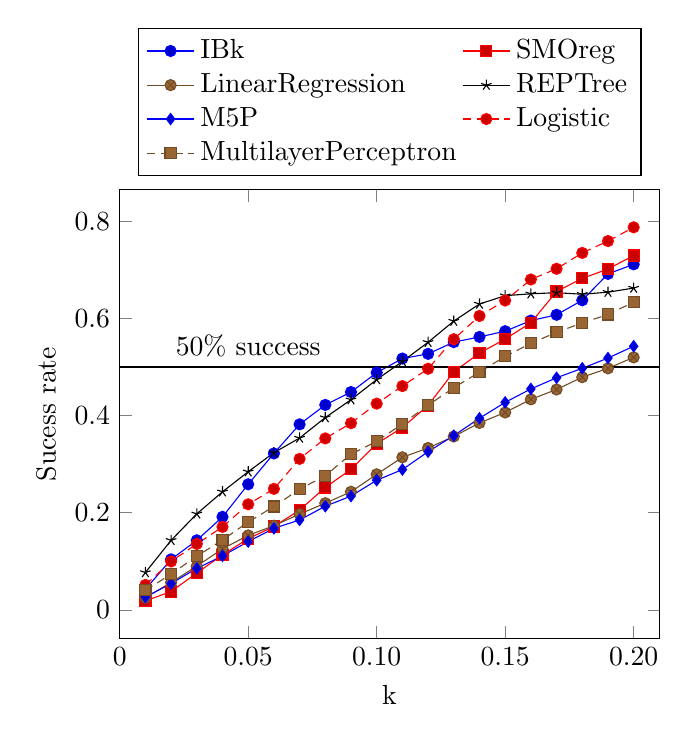
\begin{tikzpicture}
	\begin{axis}[
			%  align right:
			legend style={
				anchor=south,
				at={(0.5,1.03)}
			},
			legend columns=2,
			legend cell align=left,
			xtick={0,0.05,0.10,0.15,0.20},
			xticklabels={$0$, $0.05$, $0.10$, $0.15$, $0.20$},
			xmin=0.0,
			xmax=0.21,
			xlabel={k},
			ylabel={Sucess rate}
		]

		\addplot coordinates {(0.01, 0.042250) (0.02, 0.103900) (0.03, 0.143100) (0.04, 0.191450) (0.05, 0.258550) (0.06, 0.322050) (0.07, 0.381950) (0.08, 0.421950) (0.09, 0.448400) (0.10, 0.488400) (0.11, 0.517450) (0.12, 0.527050) (0.13, 0.551250) (0.14, 0.561950) (0.15, 0.573750) (0.16, 0.595600) (0.17, 0.607500) (0.18, 0.637450) (0.19, 0.691700) (0.20, 0.711450)};
		\addlegendentry{IBk}

		\addplot coordinates {(0.01, 0.018400) (0.02, 0.037650) (0.03, 0.075900) (0.04, 0.113050) (0.05, 0.146600) (0.06, 0.171550) (0.07, 0.205400) (0.08, 0.252050) (0.09, 0.289300) (0.10, 0.341900) (0.11, 0.375400) (0.12, 0.420850) (0.13, 0.490000) (0.14, 0.528650) (0.15, 0.557600) (0.16, 0.591000) (0.17, 0.655600) (0.18, 0.682450) (0.19, 0.701700) (0.20, 0.729550)};
		\addlegendentry{SMOreg}

		\addplot coordinates {(0.01, 0.025000) (0.02, 0.056350) (0.03, 0.090050) (0.04, 0.125600) (0.05, 0.153300) (0.06, 0.173300) (0.07, 0.197150) (0.08, 0.219550) (0.09, 0.243100) (0.10, 0.279050) (0.11, 0.314050) (0.12, 0.333300) (0.13, 0.356950) (0.14, 0.384900) (0.15, 0.406400) (0.16, 0.433450) (0.17, 0.453700) (0.18, 0.479100) (0.19, 0.497200) (0.20, 0.519850)};
		\addlegendentry{LinearRegression}

		\addplot coordinates {(0.01, 0.076900) (0.02, 0.143150) (0.03, 0.197650) (0.04, 0.243100) (0.05, 0.284350) (0.06, 0.323600) (0.07, 0.353800) (0.08, 0.395850) (0.09, 0.432650) (0.10, 0.474100) (0.11, 0.511350) (0.12, 0.550950) (0.13, 0.594500) (0.14, 0.629700) (0.15, 0.646900) (0.16, 0.650700) (0.17, 0.653050) (0.18, 0.649800) (0.19, 0.654050) (0.20, 0.662550)};
		\addlegendentry{REPTree}

		\addplot coordinates {(0.01, 0.026300) (0.02, 0.054150) (0.03, 0.085400) (0.04, 0.111000) (0.05, 0.140550) (0.06, 0.167800) (0.07, 0.185050) (0.08, 0.213300) (0.09, 0.234250) (0.10, 0.266800) (0.11, 0.288850) (0.12, 0.325550) (0.13, 0.358750) (0.14, 0.394450) (0.15, 0.427200) (0.16, 0.454850) (0.17, 0.477800) (0.18, 0.497350) (0.19, 0.518400) (0.20, 0.542750)};
		\addlegendentry{M5P}

		\addplot coordinates {(0.01, 0.051250) (0.02, 0.099650) (0.03, 0.135700) (0.04, 0.170750) (0.05, 0.217300) (0.06, 0.249050) (0.07, 0.310850) (0.08, 0.353000) (0.09, 0.384350) (0.10, 0.424600) (0.11, 0.460700) (0.12, 0.496400) (0.13, 0.557200) (0.14, 0.605150) (0.15, 0.636800) (0.16, 0.680250) (0.17, 0.702200) (0.18, 0.734900) (0.19, 0.759350) (0.20, 0.787650)};
		\addlegendentry{Logistic}

		\addplot coordinates {(0.01, 0.040100) (0.02, 0.073600) (0.03, 0.110450) (0.04, 0.143950) (0.05, 0.180750) (0.06, 0.212750) (0.07, 0.248450) (0.08, 0.276050) (0.09, 0.320650) (0.10, 0.346850) (0.11, 0.383000) (0.12, 0.421250) (0.13, 0.457300) (0.14, 0.489550) (0.15, 0.521850) (0.16, 0.548700) (0.17, 0.571500) (0.18, 0.590700) (0.19, 0.608200) (0.20, 0.633450)};
		\addlegendentry{MultilayerPerceptron}

		\addplot[no markers] coordinates {(0.00, 0.50) (0.21, 0.50)}
				node[above] at (axis cs:0.05,0.50) {50\% success};

	\end{axis}
	\end{tikzpicture}

	\caption{Success rates for different classifiers}
	\label{fig:ClassifierComparison}
\end{center}
\end{figure}

Because the increase of the success rate is not exactly linear, there is no clear best choice at first glance. However, because there is little use for an operator to be told that there is less than a 50\% chance that an estimated interval is correct, since such a statement would imply that it is in fact more likely that the real value lies outside the interval than within, we can focus on the parts of the graphs above that threshold. Above the 50\%-line there are only two classifiers that at some point have the highest success rate, the logistic regression and the REPTree, and a total of four classifiers at the top that overlap each other.

Based on these results, we selected the four classifiers with the highest success rates above the 50\% threshold to run additional experiments on. The first one was to analyze in more detail the size of the estimation errors. To do this, the same experiment as before was run, but instead of calculating success rates we instead calculated the mean squared error over 5000 runs. The results are presented in Figure \ref{fig:ClassifierMSQE}. The box contains the values between the 25\superscript{th} and 75\superscript{th} percentiles with the line inside marking the median value. The bottom and top whiskers show the 10\superscript{th} and 90\superscript{th} percentile respectively.

\begin{figure}[htb]
\begin{center}
	\begin{tikzpicture}
	\begin{axis} [xtick=data, symbolic x coords={IBk,REPTree,Logistic,SMOReg},
  table/header=false]
	    \addplot [box plot median] table {msqe.dat};
	    \addplot [box plot box] table {msqe.dat};
	    \addplot [box plot top whisker] table {msqe.dat};
	    \addplot [box plot bottom whisker] table {msqe.dat};
	\end{axis}
	\end{tikzpicture}

	\caption{Mean squared error for classifiers with highest success rate}
	\label{fig:ClassifierMSQE}
\end{center}
\end{figure}

It is interesting that logistic regression has the lowest upper limit of the box, which means most of its estimation errors are very small, however it also has the highest top whisker which implies that there are also times when estimations are completely off. IBk on the other hand has the lowest top whisker, and as such has a lower spread, even though it may not be quite as accurate as the regression in many cases. That being said, IBk still has the second lowest upper limit of its box and the lowest median. These properties put together make it an interesting choice. To give an example of what these values mean, we can mention that the median value for IBk is \(0.599 \cdot 10^{-9}\), which gives a root-mean-square deviation of 0.0024\% in the estimated click rates.

There is however another aspect of classifiers that is interesting to analyze further before drawing any final conclusions, namely performance. The four classifiers with the highest success rates above the 50\% threshold were analyzed from a timing point of view. The results are in Figure \ref{fig:ClassifierPerformanceCombinations}, where the time measured in milliseconds is shown on a logarithmic scale. The experiments were performed on a MacBook Pro with a 2.2 GHz Intel Core i7 processor and 8 GB of memory.

\begin{figure}[htb]
\begin{center}
	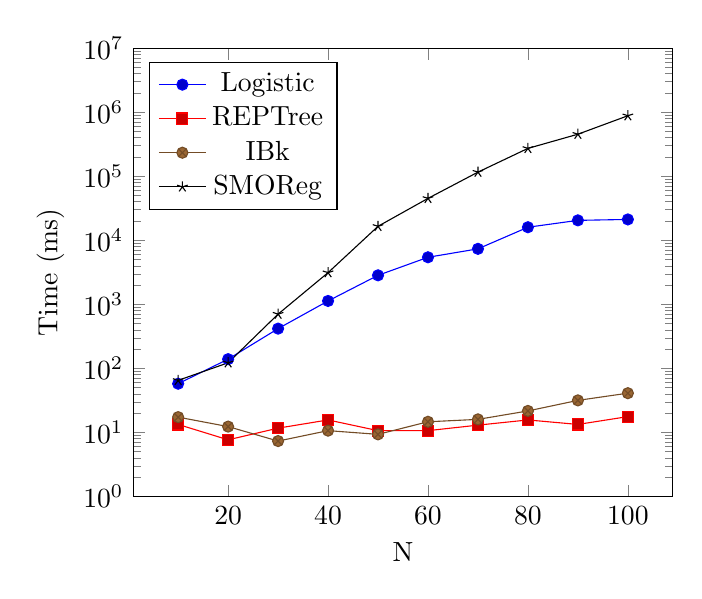
\begin{tikzpicture}
	\begin{semilogyaxis}[
			legend pos=north west,
			xlabel={N},
			ylabel={Time (ms)},
			ymin=1,
			ymax=10000000,
			clip=true
		]
		\addplot coordinates {(10, 57.666666666666664) (20, 139.33333333333334) (30, 417.6666666666667) (40, 1129.6666666666667) (50, 2838.3333333333335) (60, 5429.666666666667) (70, 7355.0) (80, 15995.333333333334) (90, 20474.666666666668) (100, 21176.0) };
		\addlegendentry{Logistic}

		\addplot coordinates {(10, 13.333333333333334) (20, 7.666666666666667) (30, 11.666666666666666) (40, 15.666666666666666) (50, 10.666666666666666) (60, 10.666666666666666) (70, 13.0) (80, 15.666666666666666) (90, 13.333333333333334) (100, 17.666666666666668) };
		\addlegendentry{REPTree}

		\addplot coordinates {(10, 17.333333333333332) (20, 12.333333333333334) (30, 7.333333333333333) (40, 10.666666666666666) (50, 9.333333333333334) (60, 14.666666666666666) (70, 16.0) (80, 21.666666666666668) (90, 31.666666666666668) (100, 41.0) };
		\addlegendentry{IBk}

		\addplot coordinates {(10, 65.0) (20, 122.33333333333333) (30, 703.3333333333334) (40, 3123.6666666666665) (50, 16532.333333333332) (60, 45116.0) (70, 115977.0) (80, 272214.6666666667) (90, 453159.0) (100, 880251.0) };
		\addlegendentry{SMOReg}
	\end{semilogyaxis}
	\end{tikzpicture}

	\caption{Classifier performance (combinations)}
	\label{fig:ClassifierPerformanceCombinations}
\end{center}
\end{figure}

For each data point, a new set of data was generated with N attribute values for two attributes (representing the body text and image used at Company A). The data set thus contained \(N^2\) instances from which N instances were removed and put into a set of test data. The removed instances were those combinations of text \(i\) and image \(j\) where \(i = j\). This systematic removal was used to guarantee that no property value would be completely removed, which could potentially happen with a random removal process. The remaining \(N(N-1)\) instances were left as the training set. Each instance in the training data was given metrics, which were drawn from a random distribution.

After this, the time taken for each classifier to initialize itself (i.e. create the underlying data model based on the training data) plus the time required to estimate the N instances from the test data was measured. This was repeated three times for every data point and the average time was calculated.

As can be seen in Figure \ref{fig:ClassifierPerformanceCombinations}, the IBk and REPTree algorithms are really fast, almost constant no matter the size of N. Then comes logistic regression which takes about 21 seconds for \(N = 100\), whereas SMO regression is highly unsuitable for larger data sets since it required more than 14 minutes at the same value for N.

Another aspect of time performance is increasing the number of occurrences of the same ad, each with its own metrics. Continuing with the previous experiment, we fixed \(N\) at 10 and added a second variable \(M\), which is the number of times each ad should occur. The reason for this experiment is to get an idea of whether it is the possible combinations or the actual number of instances which has the most impact on the time it takes to build the estimation model and estimate ads. The results are displayed in Figure \ref{fig:ClassifierPerformanceInstances}.

\begin{figure}[htb]
\begin{center}
    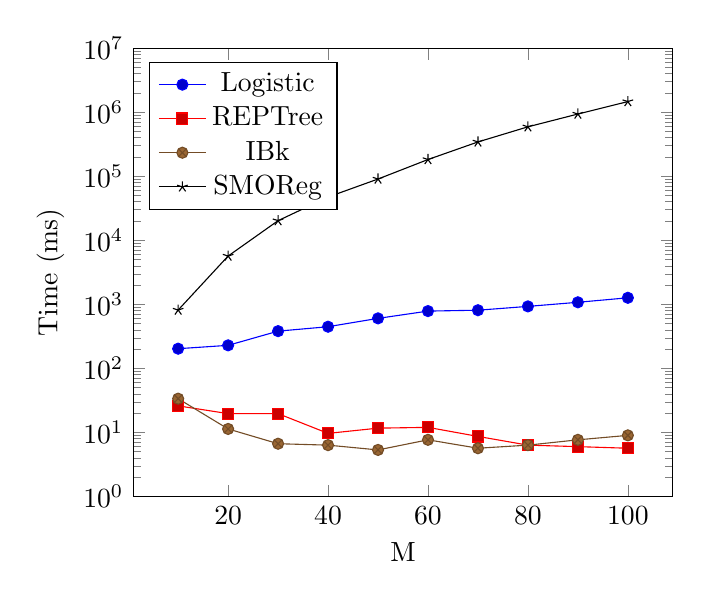
\begin{tikzpicture}
    \begin{semilogyaxis}[
            legend pos=north west,
            xlabel={M},
            ylabel={Time (ms)},
            ymin=1,
            ymax=10000000
        ]
        \addplot coordinates {(10, 203.0) (20, 229.0) (30, 381.6666666666667) (40, 447.3333333333333) (50, 604.0) (60, 784.6666666666666) (70, 810.0) (80, 929.0) (90, 1076.3333333333333) (100, 1265.3333333333333)};
        \addlegendentry{Logistic}

        \addplot coordinates {(10, 26.0) (20, 19.666666666666668) (30, 19.666666666666668) (40, 9.666666666666666) (50, 11.666666666666666) (60, 12.0) (70, 8.666666666666666) (80, 6.333333333333333) (90, 6.0) (100, 5.666666666666667) };
        \addlegendentry{REPTree}

        \addplot coordinates {(10, 33.666666666666664) (20, 11.333333333333334) (30, 6.666666666666667) (40, 6.333333333333333) (50, 5.333333333333333) (60, 7.666666666666667) (70, 5.666666666666667) (80, 6.333333333333333) (90, 7.666666666666667) (100, 9.0) };
        \addlegendentry{IBk}

        \addplot coordinates {(10, 814.6666666666666) (20, 5677.0) (30, 20249.666666666668) (40, 47347.666666666664) (50, 90509.0) (60, 182494.33333333334) (70, 343250.6666666667) (80, 591277.0) (90, 936365.3333333334) (100, 1464336.6666666667) };
        \addlegendentry{SMOReg}
    \end{semilogyaxis}
    \end{tikzpicture}

    \caption{Classifier performance (instances)}
    \label{fig:ClassifierPerformanceInstances}
\end{center}
\end{figure}

The time performance in the two experiments is comparable. The main difference is that logistic regression seems to handle the increase in the number of instances much better than the the increase in combinations of property values. Since \(M=1\) in the first experiment, there are a total of 10000 instances in the generated data set when \(N=100\), which is the same amount as the second experiment has for \(M=100\) when \(N=10\). Still, the time taken is higher by a factor of 16 for the first experiment.

The most time consuming task for the two slower algorithms is building the actual classifier. Depending on how often an organization needs to update the knowledge base, this could have an effect on the choice of classifier. The accuracy of logistic regression will outweigh the cost in time in some cases, however for large sets of data it may be more useful to suffer the slight loss in accuracy in order to efficiently incorporate new data in the model, in which case the IBk is recommended, since its mean squared error is lower than the REPTree.

For Company A we decided to use the faster IBk algorithm, because they expected to reach the limits of what logistic regression can handle without requiring so much time that it affects the user experience. Another option discussed was having functionality in the user interface to switch between algorithms, but the idea was discarded for two reasons. First of all, the data set would most likely grow fast enough so that a switch would be required very soon anyway, and secondly there was the problem of making such a function understandable for the average operator, since they are not expected to know about classification algorithms.

\subsection{Selection strategy}
Once the estimations are made the question becomes how to select which ads to run. As described in RQ 1.3, if the goal is to gain the highest average click rate over all running ads, it could perhaps be more effective to choose multiple suggested ads to minimize the impact of erroneous estimations.

Strategy N is defined as the selection strategy where the N highest estimated ads are run. In addition to this, the ads were run either weighted or unweighted. The latter means that all ads are shown the same amount of times, whereas the former approach calculates a weight for each ad based on the normalized value of the estimate. Functions for the calculations are shown in Equation \ref{eq:CUnweighted} and \ref{eq:CWeighted} respectively. This process was then repeated 5000 times and the values averaged to identify the optimal selection strategy. The results are available in Table \ref{tbl:SelectionStrategy} for both logistic regression and IBk.

\begin{equation}
	c_{unweighted} = \sum_{i=1}^{N} \frac{ c_i }{ N } \\
	\label{eq:CUnweighted}
\end{equation}
\begin{equation}
	c_{weighted} = \frac{ \sum_{i=1}^{N} \hat{c}_i \cdot c_i }{ \sum_{i=1}^{N} \hat{c}_i }
	\label{eq:CWeighted}
\end{equation}

\begin{table}
\begin{center}
	\begin{tabular}{ l || c | r  r  }
        \hline
		\textbf{Algorithm} & \textbf{N} & Unweighted & Weighted \\
		\hline
		\multirow{3}{*}{Logistic}
         & 1 & 0.0209\% & 0.0208\% \\
		 & 2 & 0.0201\% & 0.0201\% \\
		 & 3 & 0.0192\% & 0.0192\% \\
         \hline
         \multirow{3}{*}{IBk}
         & 1 & 0.0205\% & 0.0203\% \\
         & 2 & 0.0197\% & 0.0197\% \\
         & 3 & 0.0190\% & 0.0190\% \\
		\hline
	\end{tabular}
	\caption{Averaged real click rate for selection strategies N}
	\label{tbl:SelectionStrategy}
\end{center}
\end{table}

As the results reveal, the best approach over time from a purely statistical point of view is to only select the ad with the highest estimated performance, no matter which of the two algorithms is used. Other reasons for choosing multiple suggestions may of course exist, such as diversifying for potential target groups for example, but those choices need to be made by a domain expert. It is also interesting to note that the weighting of ads carries no additional boost nor any significant negative effect to the average performance.

While these results do not support any more complicated selection strategy than "best first" as answer to RQ 1.3, they do strengthen the proof for that the classifiers indeed provides a good estimate. A strategy where \(N > 1\) would only be better suited if the estimator tended to overestimate the value of the \(N-1\) first ads, so that in fact the N\superscript{th} was the best choice of ad. In other words, the results indicate that the ranking of the suggested ads on \(\hat{c}\) reflect the expected ranking based on \(c\).

\subsection{Influence of time}
To accurately be able to compare the estimated performance of a new ad with existing ads, it is important to also estimate future performance of already existing ads. If ad performance declines over time, even the best performing ad may reach a point in time where its performance is expected to be worse than that of a new ad. The reason for such a decline could be for example because the advertiser will not show a specific ad to a user who has previously clicked it.

In order to be able to analyze this question, described in RQ 1.4, data was collected daily over a period of two weeks for two separate ads, one targeting men and one targeting women. The reason for choosing two weeks was a trade-off between being able to identify differences between weekdays and those over time (e.g. perhaps weekends see a higher performance due to an increase in online presence) while not incurring too high costs.

The performance for the ads is presented in Figure \ref{fig:TimeInfluence1} and \ref{fig:TimeInfluence2} respectively. The dots represent the mean click rate for each day, whereas the bars on each coordinate represent the 90\% confidence interval for the click rate. We can calculate this interval since we have made the assumption that the data is normally distributed, as was described in the data set description. The values on the x-axis is the day of the week of the measurement. The data was collected between October 3\superscript{rd} and October 17\superscript{th} 2012. It is worth mentioning that October 12, the second Friday in the data set, was a holiday in the targeted region.

\begin{figure}[htb]
\begin{center}
	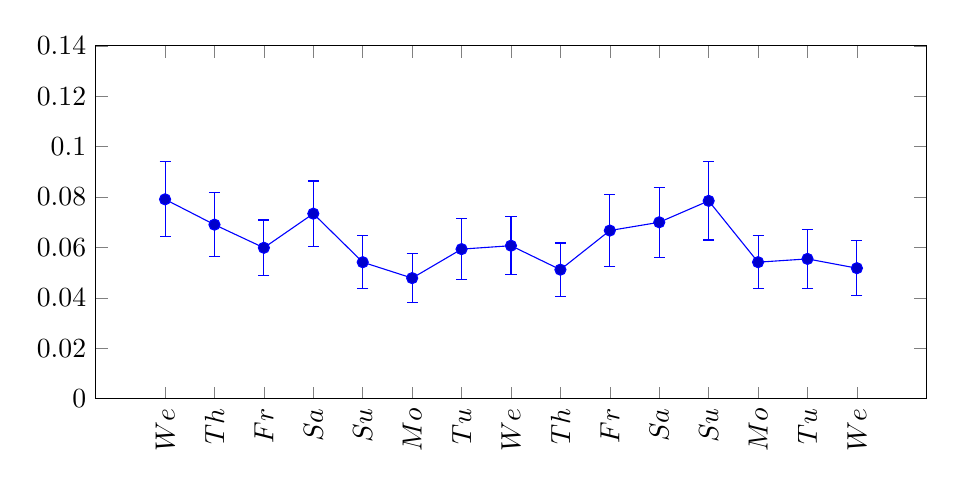
\begin{tikzpicture}
	\begin{axis}[
			%  align right:
			legend style={
				cells={anchor=east},
				legend pos=outer north east,
			},
			legend cell align=left,
			width=\linewidth,
			height=0.5\linewidth,
            ymin=0.0,
			ymax=0.14,
            ytick={0.0,0.02,...,0.14},
			y tick label style={/pgf/number format/fixed},
			xtick=data,
			xticklabels={$We$,$Th$,$Fr$,$Sa$,$Su$,$Mo$,$Tu$,$We$,$Th$,$Fr$,$Sa$,$Su$,$Mo$,$Tu$,$We$},
			x tick label style={rotate=90,anchor=east},
		]

		\addplot+[error bars/.cd, y dir=both,y explicit] coordinates {
			%(2, 0.08295) +- (0, 0.01746)
			(3, 0.07909) +- (0, 0.01492)
			(4, 0.06904) +- (0, 0.01277)
			(5, 0.05986) +- (0, 0.01101)
			(6, 0.07341) +- (0, 0.01294)
			(7, 0.05414) +- (0, 0.01049)
			(8, 0.04783) +- (0, 0.00968)
			(9, 0.05933) +- (0, 0.01210)
			(10, 0.06069) +- (0, 0.01152)
			(11, 0.05118) +- (0, 0.01060)
			(12, 0.06670) +- (0, 0.01416)
			(13, 0.06998) +- (0, 0.01395)
			(14, 0.07848) +- (0, 0.01554)
			(15, 0.05415) +- (0, 0.01049)
			(16, 0.05545) +- (0, 0.01158)
			(17, 0.05177) +- (0, 0.01099)
			%(18, 0.04937) +- (0, 0.01624)
		};

	\end{axis}
	\end{tikzpicture}

	\caption{CTR over time for ad targeting women}
	\label{fig:TimeInfluence1}
\end{center}
\end{figure}

\begin{figure}[htb]
\begin{center}
	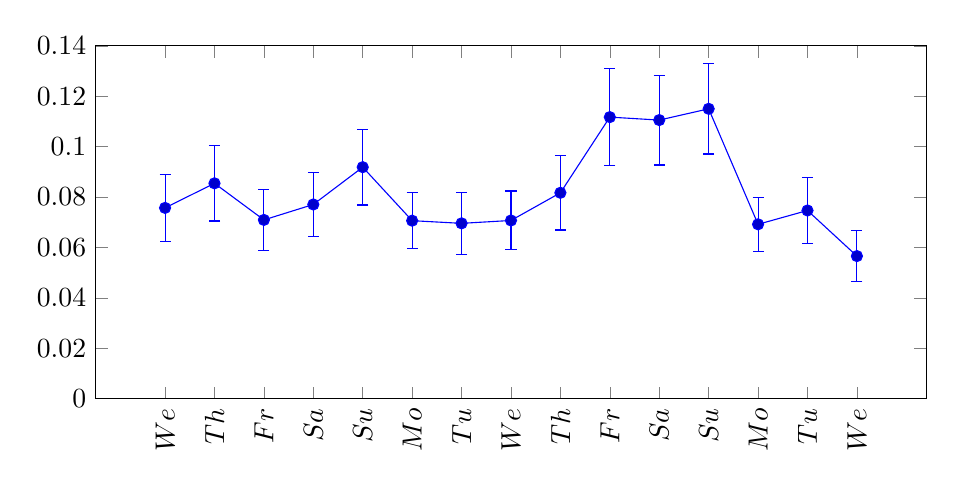
\begin{tikzpicture}
	\begin{axis}[
			%  align right:
			legend style={
				cells={anchor=east},
				legend pos=outer north east,
			},
			legend cell align=left,
			width=\linewidth,
			height=0.5\linewidth,
            y tick label style={/pgf/number format/fixed},
            ymin=0.0,
			ymax=0.14,
            ytick={0.0,0.02,...,0.14},
			xtick=data,
			xticklabels={$We$,$Th$,$Fr$,$Sa$,$Su$,$Mo$,$Tu$,$We$,$Th$,$Fr$,$Sa$,$Su$,$Mo$,$Tu$,$We$},
			x tick label style={rotate=90,anchor=east},
		]

		\addplot+[error bars/.cd, y dir=both,y explicit] coordinates {
			%(2, 0.08791) +- (0, 0.01779)
			(3, 0.07569) +- (0, 0.01334)
			(4, 0.08544) +- (0, 0.01497)
			(5, 0.07092) +- (0, 0.01216)
			(6, 0.07705) +- (0, 0.01280)
			(7, 0.09185) +- (0, 0.01503)
			(8, 0.07062) +- (0, 0.01102)
			(9, 0.06956) +- (0, 0.01226)
			(10, 0.07070) +- (0, 0.01168)
			(11, 0.08168) +- (0, 0.01474)
			(12, 0.11171) +- (0, 0.01936)
			(13, 0.11053) +- (0, 0.01782)
			(14, 0.11500) +- (0, 0.01794)
			(15, 0.06918) +- (0, 0.01070)
			(16, 0.07466) +- (0, 0.01294)
			(17, 0.05657) +- (0, 0.01015)
			%(18, 0.05035) +- (0, 0.01537)
		};

	\end{axis}
	\end{tikzpicture}

	\caption{CTR over time for ad targeting men}
	\label{fig:TimeInfluence2}
\end{center}
\end{figure}

By following the performance over the three Wednesdays in the data set, both ads do show a declining trend. It is not enough however to draw any strong conclusions on, since the confidence intervals are overlapping for all three data points in both sets. Comparing only two data points shows no strong decline, and in the case of for example Sundays there is a strong increase in both data sets. The biggest differences appear in Figure \ref{fig:TimeInfluence2}, where it becomes clear that with 90\% confidence there was an increase in click rate between Fridays.

There is some indication that given a longer time period there might be a decline, though this experiment cannot prove such a theory.

\subsection{User interface}
A graphical user interface was developed to make it easier for an operator to use the system, without dealing with command-lines and doing research into classification. Perhaps the most interesting components are the ones used for targeting (top left) and filtering (bottom), as shown in the screenshot in Figure \ref{fig:GUI}.

\begin{figure}[htb]
    \centering
    \includegraphics[width=\columnwidth]{gui-screenshot-mock-data.png}
    \caption{Graphical user interface}
    \label{fig:GUI}
\end{figure}

The available targets are automatically loaded from the underlying knowledge base (which is stored in a SQLite database), which means the operator can easily specify which data is used for suggesting new ads. For Company A, gender and age were the only targeting options used, but this could of course be extended further.

The filtering was added to limit which data is shown to the operator, since data sets will quickly become very large. Here they can choose to see either suggested ads, existing ads or both. The text box is used for free text filtering, so that it is easy to only show ads that use for example a specific image.

There are also buttons for showing average click rate for each image and each text respectively, in order to quickly get an idea of which properties leads to high performing ads. Another implemented feature was multiple knowledge bases which is useful for managing data sets that should not have any effect on each other, for example ads targeting countries with different languages.

\newpage
\section{Conclusion}
\label{ch:Conclusion}
In this thesis we have shown a technique for developing an automated system that provides decision support to organizations working with social network marketing. We have also described and performed experiments which validate our solution. Below is a summary of our results for each research question, as well as a brief description of the suggested software architecture.

\textit{\textbf{RQ 1.1.} Do ad properties have differing impact on performance?}
We clearly demonstrated how individual ad properties differ in their performance impact. In our case, the image of an ad had an overall higher correlation to the performance than the text.

\textit{\textbf{RQ 1.2.} How well do classifiers perform in estimating click rates?}
The experiments indicated that the most accurate estimator for ad click rates was the logistic regression, however a performance analysis revealed that it might be too slow for large data sets. For such a case, a faster algorithm such as the IBk is recommended, which does not suffer from the same exponential increase in time while still retaining a useful level of accuracy.

\textit{\textbf{RQ 1.3.} Which ad selection strategy provides the highest average click rate?}
The average performance did not increase by running more than one of the estimated ads. Rather, the most effective strategy for an operator to select ads to run from a list of suggestions is to choose the ad with the highest estimated performance. This is also an indication of the aptness of the classifier approach.

\textit{\textbf{RQ 1.4.} How does time affect the performance of ads?}
The experiment consisted of two weeks worth of data, but no decline in performance could be identified with any statistical certainty. We did not however rule out that such a decline may exist when analyzing a data set covering a longer time span.

The software solution consists of three basic components. The Data Manager is responsible for interacting with the knowledge base of all previously collected information. This data is then used by the Estimator, which models the data in order to provide estimates of new ads. The ads to be estimated are generated by the Ad Factory, and typically does so by generating combinations of ad properties which do not exist in the knowledge base. To interact with the system, these components need to be combined in a user interface, which most likely will be graphical though that is not a requirement.

The next subsection will discuss possible concerns regarding the validity of the research shown in this paper, followed by possible future work to extend and improve upon this work.

\subsection{Validity}
Though great care has been taken to be thorough in the research for this thesis, this section will discuss some factors that may be of interest for the reader to both understand potential limitations of the research in terms of constraints and risk factors, as well as potential future additions to the results presented in the paper.

\subsubsection{Constraints}
Running ads through a publisher obviously incurs a cost in terms of both money and time, and as such it became a constraint for this study, which of course is not in any way an unusual limitation. It was sometimes possible to use existing ad data, while at other times it was necessary to specify requirements which were passed along to the marketing department and put online. The time ads could be kept online was a trade-off between the needs of this study and the budget of Company A. The existing data sets were very useful, but in an optimal study there would be a larger set of data with long running ads, including low-performing ads that for business reasons are typically removed quickly.

\subsubsection{Risk factors}
Because the output of the system is dependent on historical data, an assumption has been made that older data is still representative of the current state of the marketing. This is definitely not true for campaigns that are adapted for Christmas, Valentine's Day or other special occasions. The assumption is that the amount of such time-dependent data is so small that it will not impact the final results. If however there is reason to believe that this set of data would influence the output, the recommended approach is to remove it from the knowledge base.

\subsection{Future work}
Due to circumstances described in the introduction, the targeting of ads was removed as a goal of this thesis. For advertisers with many campaigns with differing targeting it would most likely be interesting to extend the system with capabilities to handle target groups. For targeting which is considered binary (either a person has the attribute, or they do not), such as for example gender or nationality, the described system can be used by simply separating the data sets from each other. This is a simple solution which has the downside of not modeling potential similarities in behavior between groups, which could increase the efficiency of the modeling.

A more advanced variant of the above problem is that of attributes which can be described using scalar values. An example of this could be age, where it would be reasonable to expect that people whose age is only a year or two apart would be attracted to the same properties in an ad. Simply dividing the data sets by age would probably lead to an even greater loss of information than the cases described previously.

Though this thesis has limited the scope of the system for use with social networks, it would be useful to develop the technique further to deal with multiple classes of advertisement, such as for example search and contextual advertisement, since many organization combine classes to expand their audience.

Finally, in the discussion regarding the impact of different properties, the idea that the gender of a marketing expert could strongly influence how well ads perform was presented. This could very well be the hypothesis of future work in the field of marketing.

\section{Acknowledgements}
We would like to thank our thesis supervisor Matthias Tichy for his support and the ideas he provided throughout the project. We would also like to thank our industrial supervisor as well as the marketing people at Company A for sharing their knowledge and giving us feedback on our work.

\bibliographystyle{abbrv}
\bibliography{references} % references.bib

% Appendices
\end{document}